\chapter{Learning $\omega-$Regular Expressions}


In this chapter, we present SAT-based learning algorithm for learning $\omega-$Regular expressions from a sample of positive and negative infinite words. 

\section{$\omega$-Regular expression}
An $\omega$-regular expression $r_\omega$ is an expression with the following grammar:
\begin{equation*}
    r_\omega:=r^\omega \mid r\circ_\omega r_\omega \mid r_\omega+_\omega r_\omega
\end{equation*}
where, $r$ is a regular expression as described in Section~\ref{subsec:regex-def}. Let the set of $\omega-$regular expressions be denoted by $\mathcal{R}_{\Sigma}^{\omega}$.
Again here, a $\omega-$regular expression can be represented in the form of a syntax tree or a syntax DAG, similar to ones for regular expressions. The only difference here is that the nodes of the syntax tree and the syntax DAG are labelled by elements from $\Lambda_\omega=\Lambda\cup\{\omega, +_\omega, \circ_\omega\}$.  The semantics of a $\omega-$regular expression is as usual defined as the language they defined, which is obtained in the following manner:
\begin{equation*}
    \sema{r^\omega}=\sema{r}^\omega;\ \sema{r\circ_\omega r_\omega}=\sema{r}\circ_\omega\sema{r_{\omega}};\ \sema{r_\omega+_{\omega}r_\omega^{\prime}}=\sema{r_\omega}\cup \sema{r_\omega^{\prime}}
\end{equation*}
It should be noted that $r^\omega$ is well defined only when $\epsilon\notin \sema{r}$, since otherwise, $\sema{r^\omega}$ might contain invalid infinite words.
Now, let us look at some results regarding membership of ultimately periodic words in languages defined by $\omega-$regular expressions. In the following results, we assume $u$ and $v$ are words in $\Sigma^*$ and $r$ is a regular expression in $\mathcal{R}_\Sigma$, such that $\epsilon\notin \sema{r}$. Moreover, assume that the minimal DFA of $\sema{r}$ has size $n$.

\begin{prop}{\label{prop:w-membership}}
$uv^{\omega}\in \sema{r^{\omega}}\iff \exists i, j\in \mathbb{N},\ \abs{u}<i<j,\ uv^\omega[0,i)\in \sema{r^+}  \text{ and } uv^\omega[i,j) \in \sema{r^+} \text{ where } j\equiv i\mod \abs{v}$.
\end{prop}
\begin{proof}
 ($\Rightarrow$) From the semantics of $\omega$-regular expressions, we have $uv^\omega\in \sema{r^\omega}\implies uv^\omega\in\sema{r}^\omega$. Hence, there exists an infinite sequence of natural numbers $i_1, i_2, i_3, \ldots$ satisfying ${\abs{u}<i_1<i_2<\ldots}$ such that $uv^\omega[0,i_1)\in \sema{r^+}$ and from then on $uv^\omega[i_1,i_2)\in \sema{r}$, $uv^\omega[i_2,i_3)\in \sema{r}$ and so on. Since, $i_0,i_1,i_2, \ldots$ is an infinite sequence, it is possible to find numbers $i$ and $j$ in the sequence, such that $j\equiv i \mod \abs{v}$ using pigeonhole principle. Now, clearly, $uv^\omega[0,i)\in \sema{r^+}$ and $uv^\omega[i,j)\in \sema{r^+}$, since $i$ and $j$ belong to the sequence.

($\Leftarrow$) Let $uv^\omega[0,i)=v_1$ and $uv^\omega[i,j)=v_2$, where both $uv^\omega[0,i)$ and $uv^\omega[i,j)$ satisfy the properties mentioned in the lemma. It is an easy observation that $v_1v_2^{\omega}=uv^\omega$. As we already know ${v_1\in \sema{r^+}}$ and $v_2\in \sema{r^+}$, we can conclude that ${v_1v_2^\omega \in \sema{r^+}\circ \sema{r^+}^\omega \implies v_1v_2^\omega
\in\sema{r^\omega}\implies uv^\omega \in \sema{r^\omega}}$. 
\end{proof}
\begin{lemma}\label{lem:bound-r}
$v^{\omega}\in \sema{r^\omega}\iff\exists i \in \mathbb{N},\ v^\omega[0,i)\in \sema{r^{\abs{v}+1}}$.
\end{lemma}

\begin{proof}
$(\Rightarrow)$  Since, $v^\omega\in \sema{r}^\omega$, for any natural number $n$, there is a prefix $v^\omega[0,i)$ of $v^\omega$ such that $v^\omega[0,i)\in \sema{r^n}$. Therefore, it holds true for $n=\abs{v}+1$ as well.

($\Leftarrow$) Here, we have $v^\omega[0,i)\in \sema{r^{\abs{v}+1}}$ for some $i\in \mathbb{N}$. Therefore, we can find a finite sequence of distinct natural numbers $i_1, i_2, \ldots, i_{\abs{v}+1}$, where $i_{\abs{v}+1}=i$ and also, $v^\omega[0,i_1)\in \sema{r}$, $v^\omega[i_1,i_2)\in \sema{r}$ and so on. Now, notice that it is possible to find numbers $i^{\prime}$, $j^{\prime}$ with $i^\prime<j^\prime$, in the sequence such that $j^{\prime}\equiv i^{\prime} \mod \abs{v}$ using pigeonhole principle(Since, the sequence contains more than $\abs{v}$ elements). Consequently, we have $v^\omega[0,i^{\prime})\in\sema{r^+}$, $v^\omega[i^{\prime},j^{\prime})\in\sema{r^+}$ and $j^{\prime}\equiv i^{\prime} \mod \abs{v}$, which gives us $v^\omega\in\sema{r^\omega}$ straightaway using Prop.~\ref{prop:w-membership}.
\end{proof}
\begin{corollary}\label{cor:bound-r-uv}
Let $uv^{\omega}\in \sema{r^\omega}$ such that for some $i> \abs{u}$, $uv^\omega[0,i)\in\sema{r}$ and $uv^\omega[i,\infty)\in\sema{r^\omega}$. Then, $\exists j \in \mathbb{N},\ j>i,$ such that $uv^\omega[0,j)\in \sema{r^{\abs{v}+1}}$
\end{corollary}
The proof for this proceeds exactly the same way as Lemma~\ref{lem:bound-r}. The next lemma shows how the length of each match can be bounded.
\begin{figure}
    \centering
\tikzset{every picture/.style={line width=0.75pt}} %set default line width to 0.75pt        

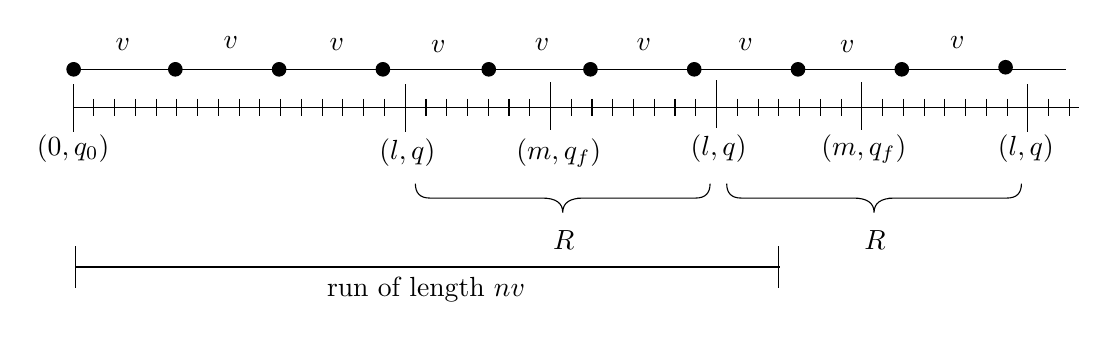
\begin{tikzpicture}[x=0.75pt,y=0.75pt,yscale=-1,xscale=1]
%uncomment if require: \path (0,300); %set diagram left start at 0, and has height of 300

%Straight Lines [id:da9738540502468893] 
\draw    (101,125) -- (585.5,125) (111,121) -- (111,129)(121,121) -- (121,129)(131,121) -- (131,129)(141,121) -- (141,129)(151,121) -- (151,129)(161,121) -- (161,129)(171,121) -- (171,129)(181,121) -- (181,129)(191,121) -- (191,129)(201,121) -- (201,129)(211,121) -- (211,129)(221,121) -- (221,129)(231,121) -- (231,129)(241,121) -- (241,129)(251,121) -- (251,129)(261,121) -- (261,129)(271,121) -- (271,129)(281,121) -- (281,129)(291,121) -- (291,129)(301,121) -- (301,129)(311,121) -- (311,129)(321,121) -- (321,129)(331,121) -- (331,129)(341,121) -- (341,129)(351,121) -- (351,129)(361,121) -- (361,129)(371,121) -- (371,129)(381,121) -- (381,129)(391,121) -- (391,129)(401,121) -- (401,129)(411,121) -- (411,129)(421,121) -- (421,129)(431,121) -- (431,129)(441,121) -- (441,129)(451,121) -- (451,129)(461,121) -- (461,129)(471,121) -- (471,129)(481,121) -- (481,129)(491,121) -- (491,129)(501,121) -- (501,129)(511,121) -- (511,129)(521,121) -- (521,129)(531,121) -- (531,129)(541,121) -- (541,129)(551,121) -- (551,129)(561,121) -- (561,129)(571,121) -- (571,129)(581,121) -- (581,129) ;


%Straight Lines [id:da13702797169170655] 
\draw    (101,114) -- (101,137) ;


%Straight Lines [id:da8041648978491207] 
\draw    (261,114) -- (261,137) ;


%Straight Lines [id:da6595616096690307] 
\draw    (411,112) -- (411,135) ;


%Straight Lines [id:da3060502963477655] 
\draw    (331,113) -- (331,136) ;


%Shape: Brace [id:dp2255019364812435] 
\draw   (265.89,161.78) .. controls (265.89,166.45) and (268.22,168.78) .. (272.89,168.78) -- (326.89,168.78) .. controls (333.56,168.78) and (336.89,171.11) .. (336.89,175.78) .. controls (336.89,171.11) and (340.22,168.78) .. (346.89,168.78)(343.89,168.78) -- (400.89,168.78) .. controls (405.56,168.78) and (407.89,166.45) .. (407.89,161.78) ;

%Straight Lines [id:da2372877431070176] 
\draw    (561,114) -- (561,137) ;


%Straight Lines [id:da10606170516071167] 
\draw    (481,113) -- (481,136) ;


%Straight Lines [id:da6169757431905829] 
\draw    (441,192) -- (441,212) ;


%Straight Lines [id:da5979976123216078] 
\draw    (102.5,202) -- (441.5,202) ;



%Straight Lines [id:da6446637744519785] 
\draw    (102,192) -- (102,212) ;


%Shape: Brace [id:dp7367618017805307] 
\draw   (415.89,161.78) .. controls (415.89,166.45) and (418.22,168.78) .. (422.89,168.78) -- (476.89,168.78) .. controls (483.56,168.78) and (486.89,171.11) .. (486.89,175.78) .. controls (486.89,171.11) and (490.22,168.78) .. (496.89,168.78)(493.89,168.78) -- (550.89,168.78) .. controls (555.56,168.78) and (557.89,166.45) .. (557.89,161.78) ;

%Straight Lines [id:da5097494136295723] 
\draw    (100.5,106.75) -- (579.5,106.75) ;


%Shape: Circle [id:dp7181991198411304] 
\draw  [color={rgb, 255:red, 0; green, 0; blue, 0 }  ,draw opacity=1 ][fill={rgb, 255:red, 0; green, 0; blue, 0 }  ,fill opacity=1 ] (98,106.75) .. controls (98,104.96) and (99.46,103.5) .. (101.25,103.5) .. controls (103.04,103.5) and (104.5,104.96) .. (104.5,106.75) .. controls (104.5,108.54) and (103.04,110) .. (101.25,110) .. controls (99.46,110) and (98,108.54) .. (98,106.75) -- cycle ;
%Shape: Circle [id:dp019890023544648194] 
\draw  [color={rgb, 255:red, 0; green, 0; blue, 0 }  ,draw opacity=1 ][fill={rgb, 255:red, 0; green, 0; blue, 0 }  ,fill opacity=1 ] (147,106.75) .. controls (147,104.96) and (148.46,103.5) .. (150.25,103.5) .. controls (152.04,103.5) and (153.5,104.96) .. (153.5,106.75) .. controls (153.5,108.54) and (152.04,110) .. (150.25,110) .. controls (148.46,110) and (147,108.54) .. (147,106.75) -- cycle ;
%Shape: Circle [id:dp8843951700933347] 
\draw  [color={rgb, 255:red, 0; green, 0; blue, 0 }  ,draw opacity=1 ][fill={rgb, 255:red, 0; green, 0; blue, 0 }  ,fill opacity=1 ] (197,106.75) .. controls (197,104.96) and (198.46,103.5) .. (200.25,103.5) .. controls (202.04,103.5) and (203.5,104.96) .. (203.5,106.75) .. controls (203.5,108.54) and (202.04,110) .. (200.25,110) .. controls (198.46,110) and (197,108.54) .. (197,106.75) -- cycle ;
%Shape: Circle [id:dp03492152069054] 
\draw  [color={rgb, 255:red, 0; green, 0; blue, 0 }  ,draw opacity=1 ][fill={rgb, 255:red, 0; green, 0; blue, 0 }  ,fill opacity=1 ] (247,106.75) .. controls (247,104.96) and (248.46,103.5) .. (250.25,103.5) .. controls (252.04,103.5) and (253.5,104.96) .. (253.5,106.75) .. controls (253.5,108.54) and (252.04,110) .. (250.25,110) .. controls (248.46,110) and (247,108.54) .. (247,106.75) -- cycle ;
%Shape: Circle [id:dp5175514544423168] 
\draw  [color={rgb, 255:red, 0; green, 0; blue, 0 }  ,draw opacity=1 ][fill={rgb, 255:red, 0; green, 0; blue, 0 }  ,fill opacity=1 ] (298,106.75) .. controls (298,104.96) and (299.46,103.5) .. (301.25,103.5) .. controls (303.04,103.5) and (304.5,104.96) .. (304.5,106.75) .. controls (304.5,108.54) and (303.04,110) .. (301.25,110) .. controls (299.46,110) and (298,108.54) .. (298,106.75) -- cycle ;
%Shape: Circle [id:dp4499225794259555] 
\draw  [color={rgb, 255:red, 0; green, 0; blue, 0 }  ,draw opacity=1 ][fill={rgb, 255:red, 0; green, 0; blue, 0 }  ,fill opacity=1 ] (347,106.75) .. controls (347,104.96) and (348.46,103.5) .. (350.25,103.5) .. controls (352.04,103.5) and (353.5,104.96) .. (353.5,106.75) .. controls (353.5,108.54) and (352.04,110) .. (350.25,110) .. controls (348.46,110) and (347,108.54) .. (347,106.75) -- cycle ;
%Shape: Circle [id:dp6528014662581125] 
\draw  [color={rgb, 255:red, 0; green, 0; blue, 0 }  ,draw opacity=1 ][fill={rgb, 255:red, 0; green, 0; blue, 0 }  ,fill opacity=1 ] (397,106.75) .. controls (397,104.96) and (398.46,103.5) .. (400.25,103.5) .. controls (402.04,103.5) and (403.5,104.96) .. (403.5,106.75) .. controls (403.5,108.54) and (402.04,110) .. (400.25,110) .. controls (398.46,110) and (397,108.54) .. (397,106.75) -- cycle ;
%Shape: Circle [id:dp7506574991528185] 
\draw  [color={rgb, 255:red, 0; green, 0; blue, 0 }  ,draw opacity=1 ][fill={rgb, 255:red, 0; green, 0; blue, 0 }  ,fill opacity=1 ] (447,106.75) .. controls (447,104.96) and (448.46,103.5) .. (450.25,103.5) .. controls (452.04,103.5) and (453.5,104.96) .. (453.5,106.75) .. controls (453.5,108.54) and (452.04,110) .. (450.25,110) .. controls (448.46,110) and (447,108.54) .. (447,106.75) -- cycle ;
%Shape: Circle [id:dp360058250991258] 
\draw  [color={rgb, 255:red, 0; green, 0; blue, 0 }  ,draw opacity=1 ][fill={rgb, 255:red, 0; green, 0; blue, 0 }  ,fill opacity=1 ] (497,106.75) .. controls (497,104.96) and (498.46,103.5) .. (500.25,103.5) .. controls (502.04,103.5) and (503.5,104.96) .. (503.5,106.75) .. controls (503.5,108.54) and (502.04,110) .. (500.25,110) .. controls (498.46,110) and (497,108.54) .. (497,106.75) -- cycle ;
%Shape: Circle [id:dp3510785942107961] 
\draw  [color={rgb, 255:red, 0; green, 0; blue, 0 }  ,draw opacity=1 ][fill={rgb, 255:red, 0; green, 0; blue, 0 }  ,fill opacity=1 ] (547,105.75) .. controls (547,103.96) and (548.46,102.5) .. (550.25,102.5) .. controls (552.04,102.5) and (553.5,103.96) .. (553.5,105.75) .. controls (553.5,107.54) and (552.04,109) .. (550.25,109) .. controls (548.46,109) and (547,107.54) .. (547,105.75) -- cycle ;

% Text Node
\draw (262,147) node  [align=left] {$\displaystyle ( l,q)$};
% Text Node
\draw (101,145) node  [align=left] {$\displaystyle ( 0,q_{0})$};
% Text Node
\draw (412,145) node  [align=left] {$\displaystyle ( l,q)$};
% Text Node
\draw (335,147) node  [align=left] {$\displaystyle ( m,q_{f})$};
% Text Node
\draw (337.39,188.78) node  [align=left] {$\displaystyle R$};
% Text Node
\draw (560,145) node  [align=left] {$\displaystyle ( l,q)$};
% Text Node
\draw (482,145) node  [align=left] {$\displaystyle ( m,q_{f})$};
% Text Node
\draw (271,213) node  [align=left] {run of length $\displaystyle n\abs{v}$};
% Text Node
\draw (487.39,188.78) node  [align=left] {$\displaystyle R$};
% Text Node
\draw (125,95) node  [align=left] {$\displaystyle v$};
% Text Node
\draw (177,94) node  [align=left] {$\displaystyle v$};
% Text Node
\draw (228,95) node  [align=left] {$\displaystyle v$};
% Text Node
\draw (277,96) node  [align=left] {$\displaystyle v$};
% Text Node
\draw (327,95) node  [align=left] {$\displaystyle v$};
% Text Node
\draw (376,95) node  [align=left] {$\displaystyle v$};
% Text Node
\draw (425,95) node  [align=left] {$\displaystyle v$};
% Text Node
\draw (474,96) node  [align=left] {$\displaystyle v$};
% Text Node
\draw (527,94) node  [align=left] {$\displaystyle v$};


\end{tikzpicture}


    \caption{The run of the DFA of $\sema{r}$ on $v^\omega[i,j)$, where $R$ is the repeating run staring at $(l,q)$. The first occurrence of $R$ happens within $n\abs{v}+1$ steps and hence, the first occurrence of state $q_f$ also happens within that many steps.}
    \label{fig:lemma3}
\end{figure}

\begin{lemma}\label{lem:bound-len_match}
$v^{\omega}[i,j)\in \sema{r}\implies \exists k\in\mathbb{N},\ k-i\leq n\abs{v} \text{ such that } v^\omega[i,k)\in \sema{r} \text{ and } k\equiv j \mod \abs{v}$, where $n$ is the size of the minimal DFA for $\sema{r}$.
\end{lemma}
\begin{proof}
If $j-i\leq n\abs{v}$, we are done, since we simply take $k=j$. On the other hand, if $j-i>n\abs{v}$, finding the suitable $k$ is a bit more involved. Firstly, since, $v^{\omega}[i,j)\in \sema{r}$, there is an accepting run of the DFA $\mathcal{A}$ for $\sema{r}$ on $v^{\omega}[i,j)$, which is of length greater than $n\abs{v}$. Now, we look at this run of $\mathcal{A}$ on $v^\omega[i,j)$. Fig \ref{fig:lemma3} provides a pictorial depiction of the run. Here we consider the run to be a sequence of tuples of the form $(m,q)$, where the first entry refers to the position in $v$ which will be read next and the second entry refers to the state of the automaton at that instant. Hence, it is easy to observe that any run longer than $n\abs{v}$ would mean that there exists a tuple which repeats itself during the run, due to pigeonhole principle. Let $(l,q)$ be the tuple which repeats itself and let the run starting at the first occurrence of $(l,q)$ to the next, be referred to as $R$. Notice that due to the deterministic nature of the automaton, $R$ repeats itself during the rest of the run. Hence, if a final state $q_f$ occurs after $n\abs{v}$ steps, there must be a tuple $(m, q_f)$ which belongs to the run $R$. Clearly, $(m, q_f)$ must have been also visited during the first occurrence of $R$, which happened within $n\abs{v}$ steps. Thus, we get a prefix $v^\omega[i,k)\in \sema{r}$, which has length less than $n\abs{v}$. Moreover, $v^\omega[i,j)$ and $v^\omega[i,k)$ terminate at the same position in $v$, meaning $k\equiv j \mod \abs{v}$.


\end{proof}

\begin{corollary}\label{cor:bound-length_match_uv}
$uv^{\omega}[i,j)\in \sema{r}, \text{ where } i<\abs{u}< j \implies \exists k\in\mathbb{N},\ \abs{u}<k\leq\abs{u}+n\abs{v} \text{ such that } uv^\omega[i,k)\in \sema{r} \text{ and } k\equiv j \mod \abs{v}$.
\end{corollary}

The proof for this statement goes along the same lines as Lemma \ref{lem:bound-len_match}. Finally, having these results, it is possible to verify whether an infinite word(ultimately periodic word in this case) actually belongs to the language of regular expression by checking only a finite portion of the word. This turns out to be useful in constructing table

\begin{theorem}{\label{thm:bounded-w-membership}}
$v^{\omega}\in \sema{r^{\omega}}\iff \exists i, j\in \mathbb{N},\ 0<i<j\leq n\abs{v}+n\abs{v}^2\ v^\omega[0,i)\in \sema{r^+}  \text{ and } v^\omega[i,j) \in \sema{r^+} \text{ where } j\equiv i\mod \abs{v}$
\end{theorem}
\begin{proof}
($\Leftarrow$) This can be seen directly from Prop.~\ref{prop:w-membership}, assuming $u=\epsilon$.

($\Rightarrow$) Using Lemma \ref{lem:bound-r}, there exists some $i^{\prime}$ such that $v^\omega[0,i^{\prime})\in \sema{r^{\abs{v}+1}}$. As a result, we can generate a sequence of distinct natural numbers, $i_1,\ldots, i_{\abs{v}+1}$, with $i_{\abs{v}+1}=i^{\prime}$ such that $v^\omega[0,i_1)\in\sema{r}$, $v^\omega[i_1,i_2)\in \sema{r}$ and so on. Now, we can find another sequence $j_1, \ldots, j_{\abs{v}+1}$ with  $j_{\abs{v}+1}$, which satisfy all the properties that the sequence of $i'$s satisfy and additionally have $j_1\leq n\abs{v}$, $j_2-j_1\leq n\abs{v}$, so on and also, $j_1\equiv i_1 \mod {\abs{v}},$ $j_2\equiv i_2 \mod \abs{v}$, so on. This is a direct consequence of Lemma \ref{lem:bound-len_match}. It is easy to see that $j_{\abs{v}}\leq n\abs{v}+n\abs{v}^2$. Moreover, we can again find some $i$ and $j$ in this sequence such that $j\equiv i \mod \abs{v}$ and clearly, $v^\omega[0,i) \in \sema{r^+}$ and $v^\omega[i,j) \in \sema{r^+}$.
\end{proof}


\begin{theorem}
$uv^\omega\in \sema{r^\omega}\iff \exists i, j\in \mathbb{N},\ \abs{u}<i<j\leq \abs{u}+n\abs{v}+n\abs{v}^2\ uv^\omega[0,i)\in \sema{r^+}  \text{ and } uv^\omega[i,j) \in \sema{r^+} \text{ where } j\equiv i\mod \abs{v}$
\end{theorem}

\begin{proof}
($\Leftarrow$) This can be seen directly from Prop. \ref{prop:w-membership}.

($\Rightarrow$) When $uv^\omega\in \sema{r^\omega}$, there could be two possible cases arising from how $uv^\omega$ matches $r^\omega$.  
\begin{itemize}[label=$-$]
    \item First case would be one in which $u\in\sema{r^+}$ and $v^\omega\in \sema{r^\omega}$. In this case, Theorem \ref{thm:bounded-w-membership} can be applied directly to obtain the result. 
    \item In the second case, $\exists i^\prime, j^\prime \in \mathbb{N}$ with $i^\prime<\abs{u}<j^\prime$, such that, $uv^\omega[0,i^\prime)\in\sema{r^+},\ uv^\omega[i^\prime,j^\prime)\in\sema{r}, \text{ and } uv^\omega[j^\prime,\infty)\in \sema{r^\omega}$. Now, it can be seen that infix $uv^\omega[i^\prime,\infty)$ satisfies the conditions of Corollary~\ref{cor:bound-r-uv}. Hence, there is some $k^\prime>j^\prime$, such that $uv^\omega[i^\prime,k^\prime)\in \sema{r^{\abs{v}+1}}$. As a result, we can generate a sequence of distinct natural numbers $i_1,\ldots, i_{\abs{v}+1}$, with $i_1=j^\prime$ and $i_{\abs{v}+1}=k^\prime$ such that $uv^\omega[i^\prime,i_1)\in\sema{r},uv^\omega[i_1,i_2)\in\sema{r}$ and so on. Combining results of  Corollary~\ref{cor:bound-length_match_uv} and Lemma~\ref{lem:bound-len_match}, we can find another sequence $j_1,j_2\ldots j_{\abs{v}+1}$ which satisfy the properties of the sequence of $i'$s and additionally have $j_1\leq\abs{u}+n\abs{v}$, $j_2-j_1\leq n\abs{v}$, $j_3-j_2\leq n\abs{v}$, so on and also, $j_1=i_1\mod{\abs{v}}$, $j_2=i_2\mod{\abs{v}}$, so on. It is easy to see that $j_{\abs{v}+1}\leq \abs{u}+n\abs{v}+n\abs{v}^2$. Moreover, in this sequence  we can find some $i$ and $j$ such that $j \equiv i \mod{\abs{v}}$ and clearly, $uv^\omega[0,i)\in\sema{r^+}$ and $uv^\omega[i,j)\in\sema{r^+}$.
\end{itemize}

\end{proof}

Motivated by the above results, we define the matching relation for infinite words which would help us to algorithmically check the matching of a ultimately periodic word with a $\omega-$ regular expression.

\begin{definition}
The matching relation $\vdash$ for finite words with regular expressions, could be extended to account for matching of ultimately periodic words with $\omega$-regular expressions as well. Here, $n$ refers to the size of the minimal DFA of $\sema{r}$ in all the cases.

 \begin{align*}
        &v^\omega[i,\infty)\vdash  r^\omega   \iff  \exists j, k\in \mathbb{N},\ i<j<k\leq i+n\abs{v}+n\abs{v}^2,\ v^\omega[i,j)\vdash r^+  \text{ and } v^\omega[j,k) \vdash r^+ \text{ where } k\equiv j\mod \abs{v}\\
    &v^\omega[i,\infty) 
    \vdash r\circ r_\omega \iff  \exists j\in \mathbb{N},\ j\leq n\abs{v},\ v^\omega[i,j)\vdash r \text{ and } v^\omega[j,\infty)\vdash r_\omega\\
    &v^\omega[i,\infty) \vdash r_\omega+ r_\omega^{\prime} \iff   v^\omega[i,\infty)\vdash r_\omega \text{ or } v^\omega[i,\infty)\vdash r_\omega^{\prime}
\end{align*}
 \begin{align*}
        &uv^\omega[i,\infty)\vdash  r^\omega   \iff  \exists j, k\in \mathbb{N},\ i+\abs{u} < j<k\leq i+\abs{u}+n\abs{v}+n\abs{v}^2,\ \\&\hspace{6.5cm} uv^\omega[i,j)\vdash r^+  \text{ and } uv^\omega[j,k) \vdash r^+ \text{ where } k\equiv j\mod \abs{v}\\
    &uv^\omega[i,\infty) \vdash r\circ r_\omega \iff  \exists j\in \mathbb{N},\ i\leq j\leq\abs{u}+ n\abs{v},\ uv^\omega[0,i)\vdash r \text{ and } uv^\omega[i,\infty)\vdash r_\omega\\
    &uv^\omega[i,\infty) \vdash r_\omega+ r_\omega^{\prime} \iff   uv^\omega[i,\infty)\vdash r_\omega \text{ or } uv^\omega[i,\infty)\vdash r_\omega^{\prime}
\end{align*}

\end{definition}
Firstly, it needs to be checked whether the matching relation satisfies ${v^\omega[i,\infty)\vdash r_\omega \iff v^\omega[i,\infty)\in \sema{r_\omega}}$.
The proof goes via induction on the structure of the the $\omega-$regular expression. 
\begin{itemize}[label=$-$]
\item \textit{Case $r_\omega=r^\omega:$} This follows directly from Theorem \ref{thm:bounded-w-membership}
\item \textit{Case $r_\omega=r\circ r^{\prime}_\omega:$} Consider the following implications:
\begin{align*}
    v^\omega[i,\infty) \vdash r\circ r^{\prime}_\omega &\iff \exists j\in \mathbb{N},\ j\leq n\abs{v},\ v^\omega[i,j)\vdash r \text{ and } v^\omega[j,\infty)\vdash r_\omega\\
    &\iff\exists j\in \mathbb{N},\ v^\omega[i,j)\in r \text{ and } v^\omega[j,\infty)\in \sema{r_\omega^{\prime}}&& \text{[Using induction hypothesis]}\\
    &\iff\exists j\in \mathbb{N},\ v^\omega[i,j)\in \sema{r} \text{ and } v^\omega[j,\infty)\in \sema{r_\omega}&& \text{[Using Lemma \ref{lem:bound-len_match}]}\\
    &\iff v^\omega[i,\infty)\in \sema{r_\omega}
\end{align*}
\item Case $r_\omega=r^{\prime}_\omega+r^{\prime\prime}_\omega:$ Consider the following implications:
\begin{align*}
        v^\omega[i,\infty) \vdash r^{\prime}_\omega + r^{\prime\prime}_\omega &\iff v^\omega[i,\infty)\vdash r_\omega \text{ or } v^\omega[i,\infty)\vdash r_\omega^{\prime}  \\
    &\iff v^\omega[i,\infty)\in \sema{r_\omega} \text{ or } v^\omega[i,\infty)\in \sema{r_\omega^{\prime}}\\
    &\iff v^\omega[i,\infty)\in \sema{r_\omega}
\end{align*}
\end{itemize}
Unlike regular expression, the construction of the tables for algorithmically checking matching of a $\omega-$regular expression with a $\omega-$word needs a slightly different approach. There are two types of tables that need to be maintained for each node 